
\begin{figure}[ht]
\centering
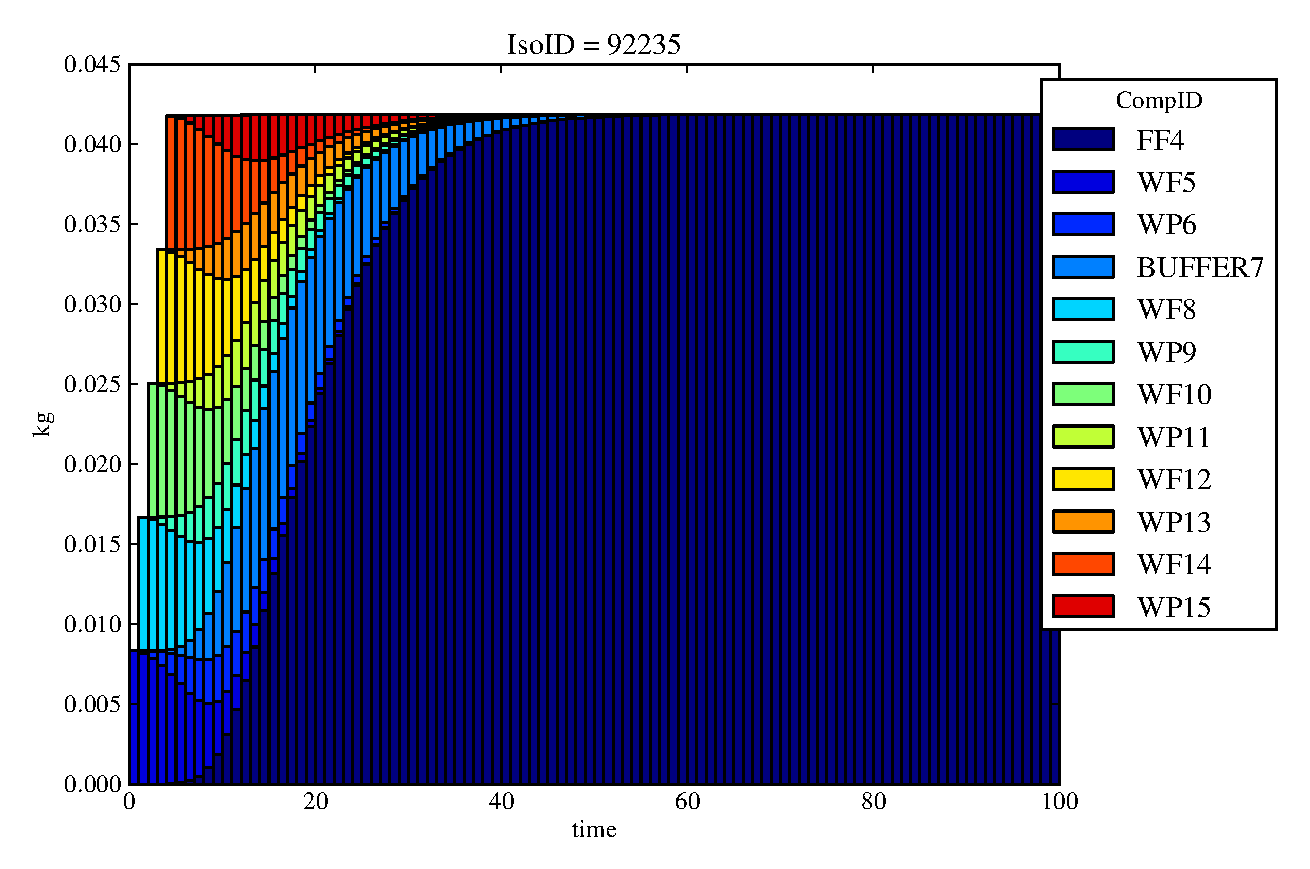
\includegraphics[width=0.6\textwidth]{./mcIII.eps}
\caption[$^{235}U$ residence. Mixed Cell Coupled Sorption and Solubility Limitation.]{
For the MCII case in which containment is affected by solubility limitation, 
($F_{d}=0.1$ for all components), $^{235}U$ travels more slowly than in the MCI case 
before permanent residence in the far field component.
}
\label{fig:mcIIIall}
\begin{minipage}[b]{0.45\linewidth}

  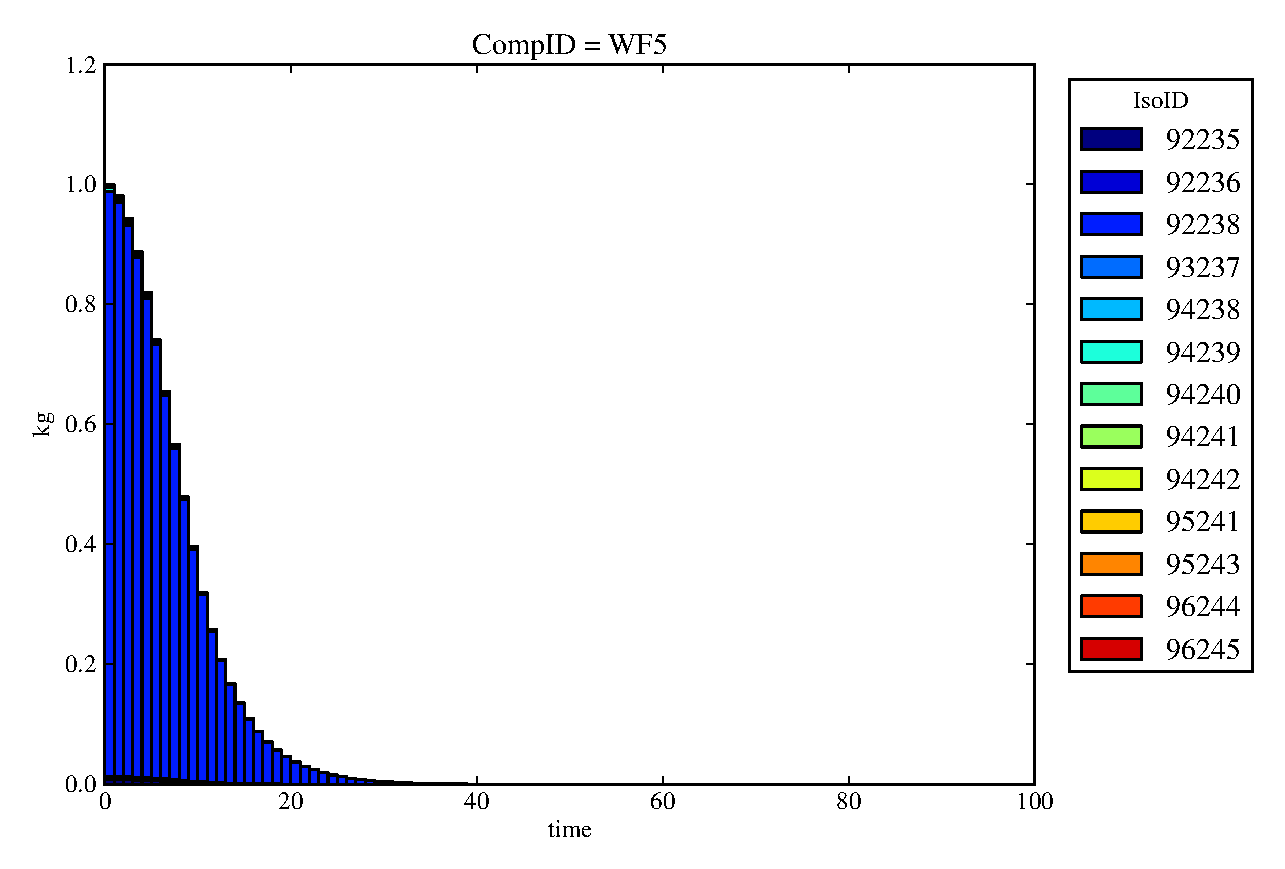
\includegraphics[width=\textwidth]{./mcIII1.eps}
  \caption[Case MCII Waste Form Contaminants.]{
    Waste Form 5 ($F_d = 0.1$, $S_{ref} = 0.001kg/m^3$) releases material with degradation. 
    }
  \label{fig:mcIIIwf5}
  
  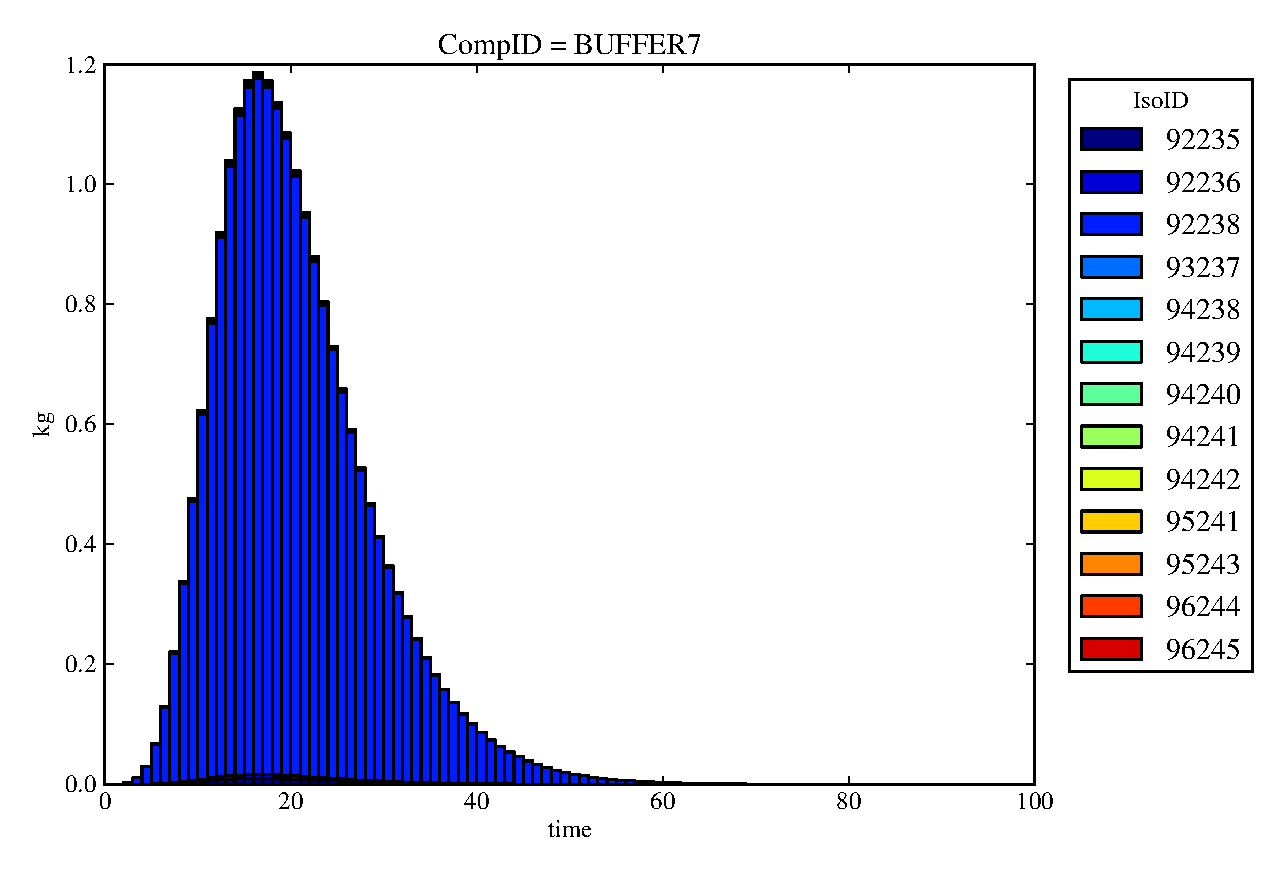
\includegraphics[width=\textwidth]{./mcIII3.eps}
  \caption[Case MCII Buffer Contaminants]{
    The Buffer, component 7 ($F_d=0.1$, $S_{ref}=0.001kg/m^3$), receives and then releases material.
    }
  \label{fig:mcIIIbuff}

\end{minipage}
\hspace{0.05\linewidth}
\begin{minipage}[b]{0.45\linewidth}
  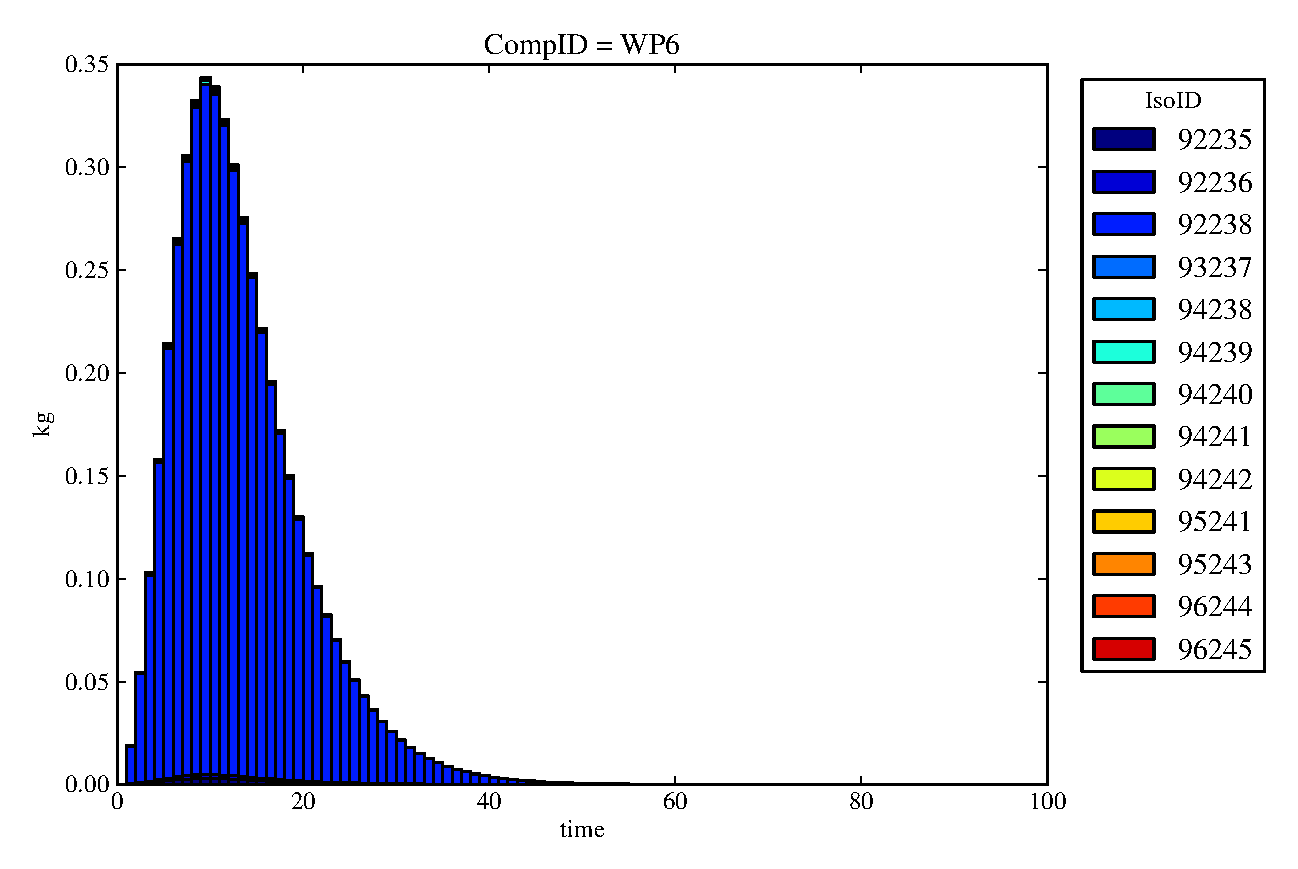
\includegraphics[width=\textwidth]{./mcIII2.eps}
  \caption[Case MCII Waste Package Contaminants.]{ 
    Waste Package 6 ($F_d = 0.1$, $S_{ref}=0.001kg/m^3$) receives then releases material. 
    }
  \label{fig:mcIIIwp6}

  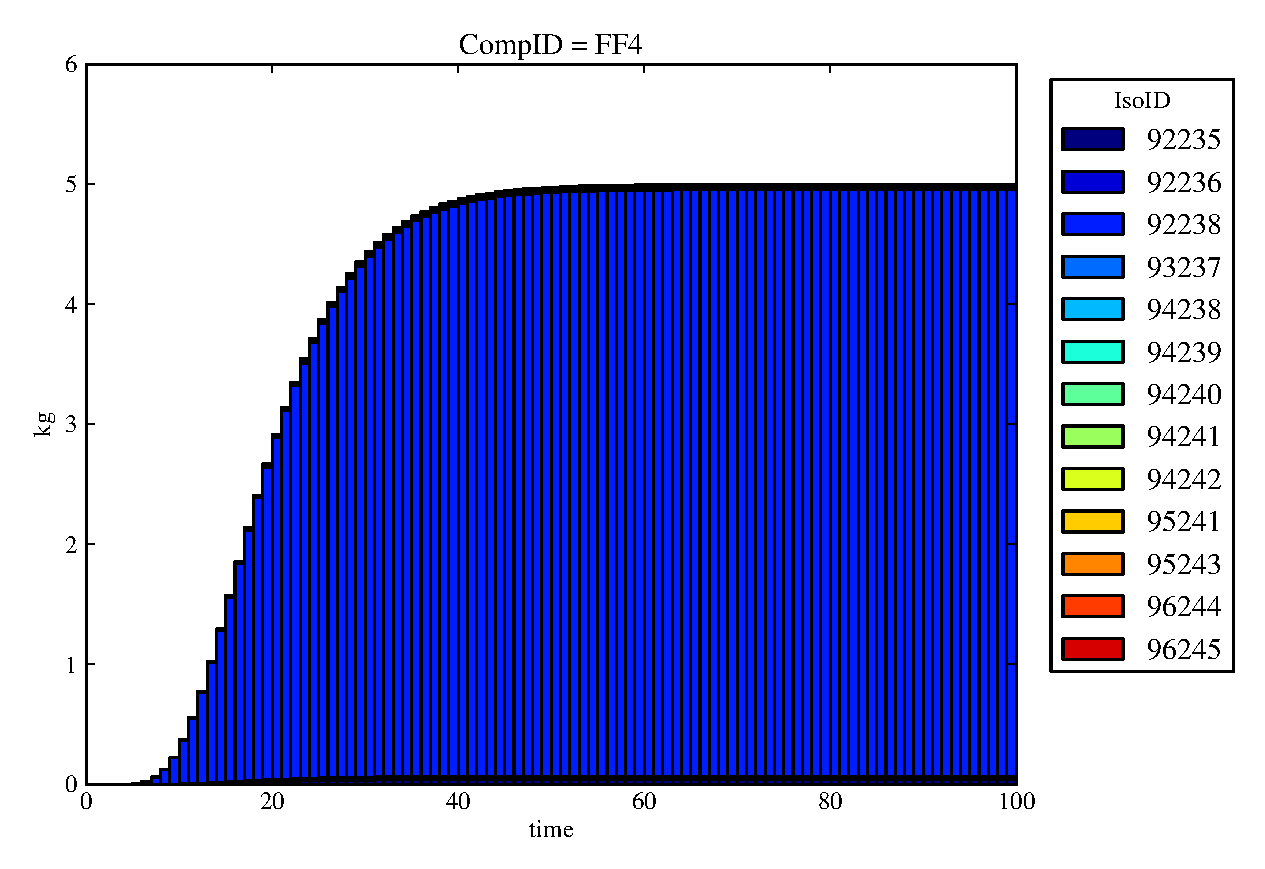
\includegraphics[width=\textwidth]{./mcIII0.eps}
  \caption[Case MCII Waste Package Contaminants.]{All material is released into 
    the Far Field, component 4 ($F_d=0.0$, $S_{ref} = 0.001kg/m^3$).}
  \label{fig:mcII}


  \end{minipage}
\end{figure}

